\chapter{Climbing the human body}
This chapter considers how DWT robots move around the human body. Attaching and moving on the human body or clothing is a challenging problem. The robots have to attach and climb on highly malleable and non-uniform surfaces.

We will discuss previous research in the area of vertical climbing robots. Afterward, we will provide experimental data and analysis of locomotion on skin and fabric with DWT robots. We focus on the exploration of skin climbing since it is a new area of research. We believe such analysis and experimentation is useful for future researchers. 

\section{Previous research}
This section looks at the previous research in climbing robots. A few robots are capable of climbing on the cloth~\cite{birkmeyer2011clash,liu2012system}. Besides this work, there are no examples of robots that climb directly on the skin. 

\subsection{Bio-inspired adhesion}
Many organisms use adhesion, so it important to look at bioinspired approaches. For light insects, it is fairly easy to climb any surface, due to a large number of tiny hairs utilizing Van Der Waals Forces or capillary forces. However, due to unfavorable scaling, larger insects, animals, and robots have to utilize a different mechanism. Although geckos appear to use Van Der Waals~\cite{autumn2002evidence}, they possess a highly sophisticated foot structure to increase surface area. Leeches~\cite{gray1938mechanism} and octopuses~\cite{laschi2009design} utilize suckers to adhere and climb vertical surfaces. Such suckers create negative pressure from muscle contractions. Some bioinspired robots have attempted to emulate such suckers, using shape memory alloy~\cite{bing2009bio} or electroactive polymers to ~\cite{bing2009bio}.

\begin{figure}[!b]
\centering
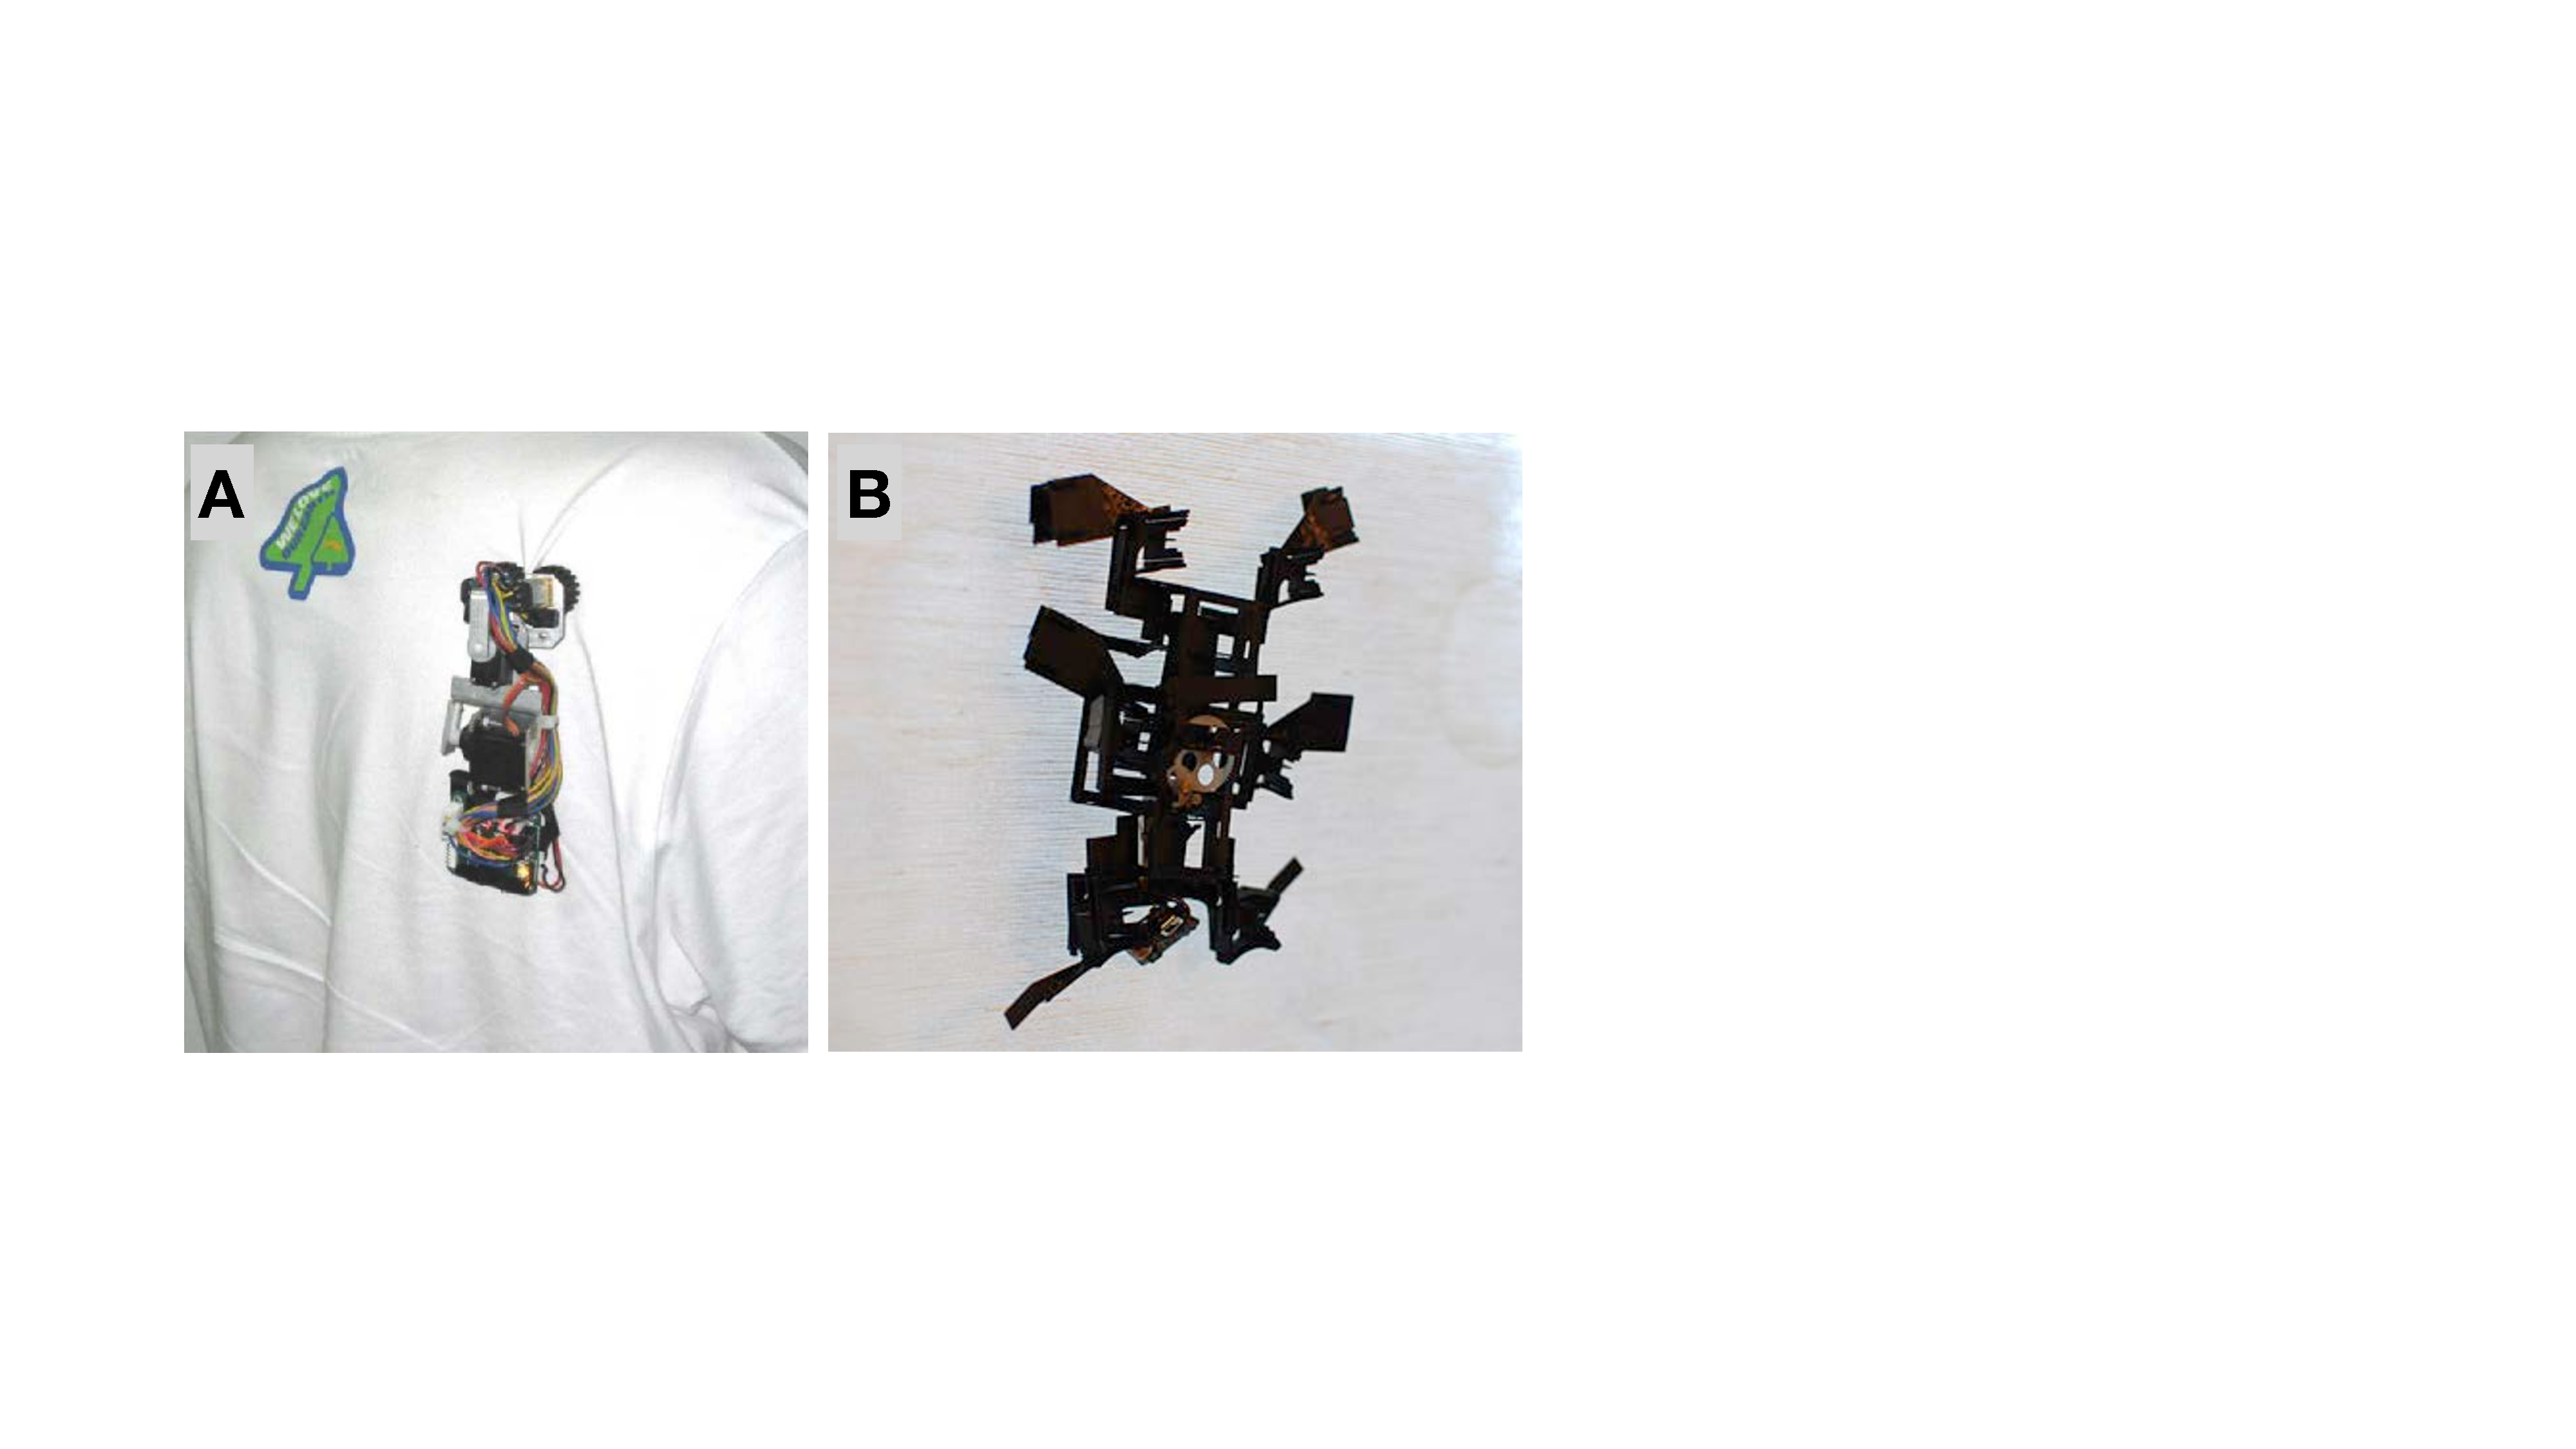
\includegraphics[width=12.0cm]{pictures/locomotion/cloth_climbing_robots.pdf}
\caption{A) Clothboth climbing on a shirt using gripper wheels. b) CLASH robot.}
\label{fig:cloth_climbing}
\end{figure}

\subsection{Cloth-climbing robots}
Although robotic fabric handling and automated sewing machines date to at least the 1980s ~\cite{briggs1988automated}. Clothing and fabric climbing robots were demonstrated in research fairly recently~(Figure~\ref{fig:cloth_climbing}). The first fabric climbing robot CLASH~\cite{birkmeyer2011clash} was made in 2011. This robot used legs with needles to penetrate and adhere to the fabric. In 2012 a cloth climbing robot Clothbot was shown~\cite{liu2012system,geng2018clothbot_beta}. It pinched the fabric between two wheels. In 2013 this project was improved and was renamed Rubbot~\cite{chen2013rubbot}. In this thesis, Rovables~\cite{dementyev2016rovables} used a different mechanism, a magnetic pinch roller on the back for fabric adhesion. 

\subsection{Wall climbing robots}
There are more examples of wall climbing robots, in contrast to cloth climbing. There are more practical applications for such robots like inspection and cleaning of inaccessible surfaces in nuclear power plants. Waalbot~\cite{murphy2007waalbot} used pressure adhesive wheels to climb vertical surfaces. Some robots used artificial gecko skin adhesive to climb surfaces~\cite{menon2004gecko}. This method uses micromachined hair-like structures to increase surface area and allow adhesion through Van der Waals forces. Other robots used vacuum suction to adhere to vertical surfaces~\cite{briones1994wall}. Another robot used tracks with permanent magnets to climb metallic surfaces~\cite{eich2011design} and grippers~\cite{lam2011flexible} to climb trees and poles. 

\subsection{Soft climbing robots}
Soft robotics is a relatively new area of robotics. Instead of using rigid bodies, soft robotics looks at highly compliant materials (e.g., silicone)~\cite{trivedi2008soft} Soft robotics are especially useful for interfacing with the human body, as they provide a close match to the compliance of the human body. Soft robots have been used to create exoskeletons~\cite{polygerinos2015soft,tsagarakis2003development}. Researchers have looked at wearable robots that can grow on the human body for providing haptic feedback~\cite{agharese2018hapwrap}. This robot wraps itself over an arm by inflating in a coil. 


\section{Robot movement on the skin}
This section evaluates the basic properties of SkinBot, such as locomotion, adhesion, and power requirements. Also, we conduct several experiments to understand some of the unique challenges of skin locomotion such as skin stretchability, its curvature, and hair presence. We also test the dead-reckoning localization method. Finally, we conduct a user study to assess the user perception of SkinBot.  

\begin{figure}[!t]
\centering
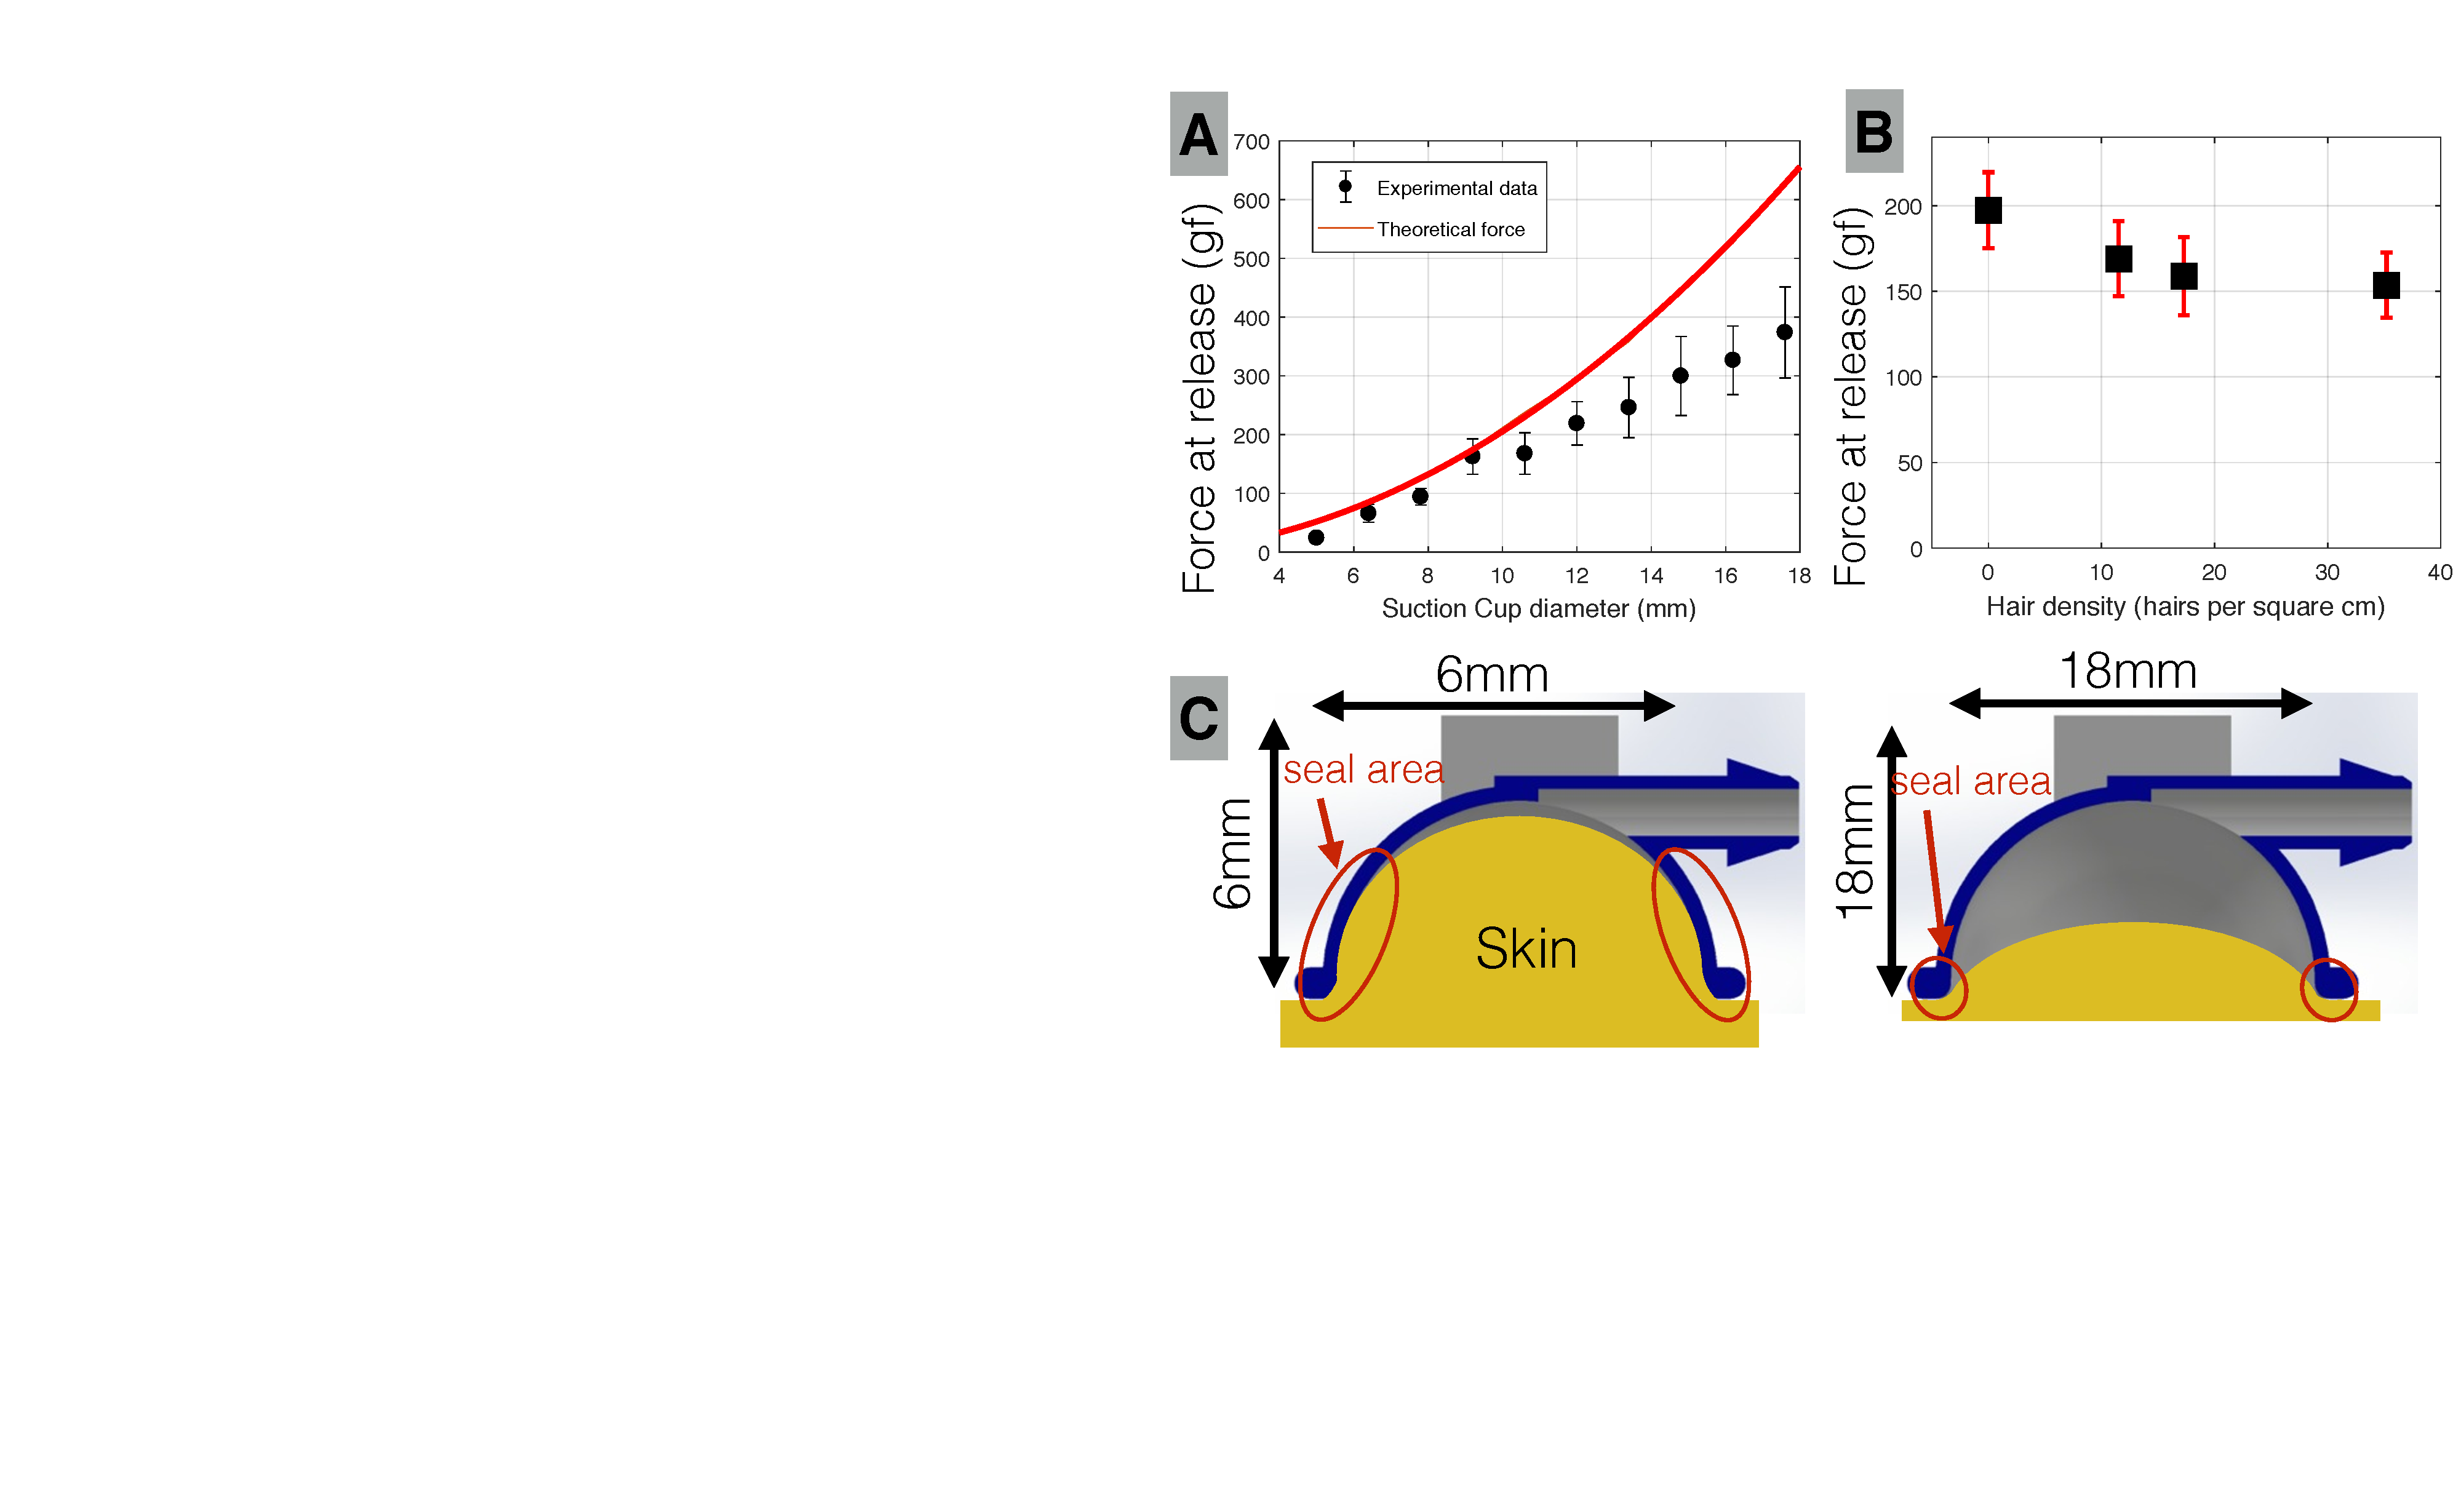
\includegraphics[width=12.0cm]{pictures/chapter3/skin_attachment_experiment.pdf}
\caption{Skin attachment experiments. A)~Maximum adhesion forces with different suction cup diameters as indicated by force at release. B)~Presence of hair on the skin reduces the maximum adhesion force. C)~Diagram illustrating the vertical displacement of the skin under suction. The suction cup of 6mm and 18mm diameters are shown in the illustration. The 6mm diameter cup creates a better cup-skin seal, as it has a larger seal area.}
\label{fig:skin_attachment_experiment}
\end{figure}

\subsection{Adhesion}
Suction provides a strong and reliable adhesion approach to the skin. In the case of SkinBot, the adhesion strength is between 150gf and 200gf when attached to a single cup and between and 300gf and 400gf when attached to the two suction cups simultaneously. This range provides enough adhesion to sustain the current weight of the robot, which is 20g. Thus, when the robot is hanging upside down, there is at least 7.5x safety factor that can be used to account for different skin types and irregularities. 

To help study adhesion, we define adhesion force as the peak force at which a suction cup pulled in the normal direction to the skin is detached from the skin. In theory, the maximum adhesion force is directly proportional to the size of the suction cup, with the governing equation: \[F=PA,~and~ A=  \pi(d/2)^2\] where $F$ is the maximum adhesion force, $P$ is the vacuum pressure, $A$ is the skin contact area of the suction cup, and $d$ is the diameter of the circular contact area. Therefore, larger suction cups have higher adhesion forces. While the theory generally agrees with \textit{in vivo} experimental data (see Figire~\ref{fig:skin_attachment_experiment}A), the suction cups over 10mm diameter consistently had lower adhesion forces than the theoretical ones. To help further understand this effect, we 3D-printed transparent suction cups with various diameters and video recorded the skin under the vacuum. After careful examination, we believe this discrepancy occurred due to two main factors. First, suction cups over 10mm have small skin-cup seal area, as shown in Figure~\ref{fig:skin_attachment_experiment}C. In other words, while the skin is displaced by the same amount for the small and large suction cups, the displacement is spread over a larger area for the larger cups. Second, larger suction cups require a more substantial seal area around its diameter. When the suction cup is being slowly pulled off, there are more chances for gaps in the seal before reaching the maximum theoretical adhesion force.  

In our experiments, we noticed that hair presence can negatively impair adhesion performance. To study this effect, we measured adhesion forces on skin surfaces with different amounts of hair (see Figure~\ref{fig:skin_attachment_experiment}B). For each of the experimental skin locations, hair density was manually counted by using a microscope. Moderate presence of hair on the skin reduces the adhesion force by around 30\% to 150 gf but still allowed attachment. Beyond that, excessive hair (above 35 hairs per cm$^2$) prevented suction cups from making the necessary skin-cup seal.

For all adhesion measurements, we used the 20N digital force gauge (DFS20, Nextech). All measurements were done on the forearm and repeated five times in different locations. The mean of the five trials was reported as a result. The attachment experiments were done on a 30-year old male. The suction cups were pulled manually, and the peak force was recorded, as the maximum pull-off force. For the measurements, the suction cups were 3D-printed with a custom force gauge attachment, so they can be pulled in a normal direction to the adhesion surface.

\begin{figure}[!b]
\centering
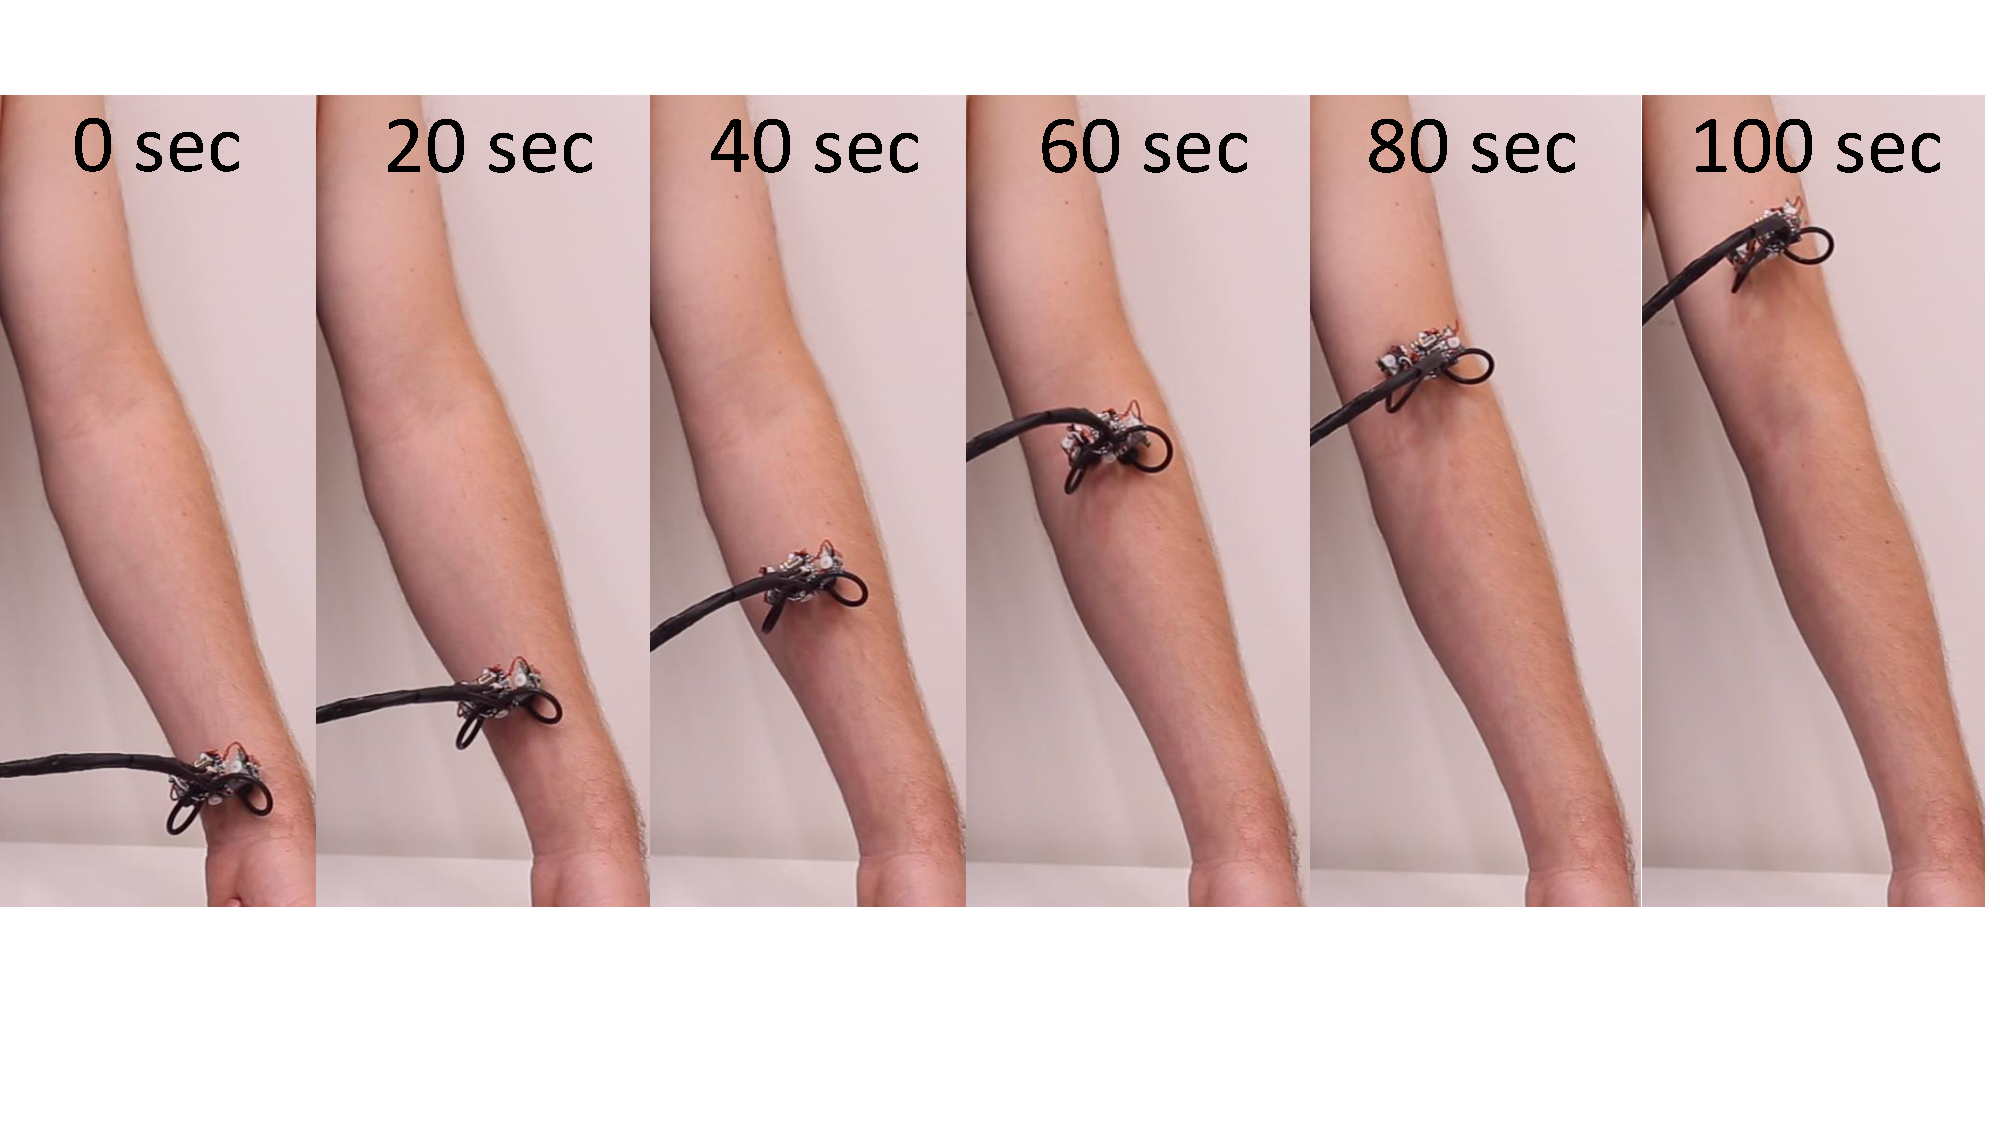
\includegraphics[width=12.0cm]{pictures/chapter3/snapshot_locomotion.pdf}
\caption{Robot locomotion on the arm. SkinBot climbing on the arm during 100 seconds.}
\label{fig:locomotion_snapshot}
\end{figure}

\subsection{Locomotion}
Figure~\ref{fig:locomotion_snapshot} shows a snapshot of the movement of SkinBot on an inclined arm. Figure~\ref{fig:locomotion_mechanism}B shows the details of air pressure changes during the locomotion. The achieved vertical climbing speed of the robot is 31cm/min with solenoid valves and 6.3cm/min without solenoid valves. However, adding the solenoid valves increases the power consumption by 50 mW, and the weight of the robot by 10g. Without the valves, the vacuum release time is around 16sec, greatly limiting the climbing speed. In particular, the robot has to wait to reach atmospheric pressure by air leakage as the servo motors are not strong enough to lift an attached cup. By opening the vacuum line to atmospheric air with a 3-way solenoid valve, the time can be significantly reduced to 0.5sec. A potential future alternative would involve using mechanical cams driven by existing actuators to break the vacuum. 

The robot can effectively walk backward by running the horizontal servos in reverse mode. The robot can rotate 30$^o$ in 20 milliseconds to change its direction. Due to the possible tangling of vacuum tubes, the rotation radius has been limited to be between -30$^o$ and 30$^o$ per locomotion step. By combining multiple steps, the robot can potentially rotate to any angle.  



\begin{figure}[!ht]
\centering
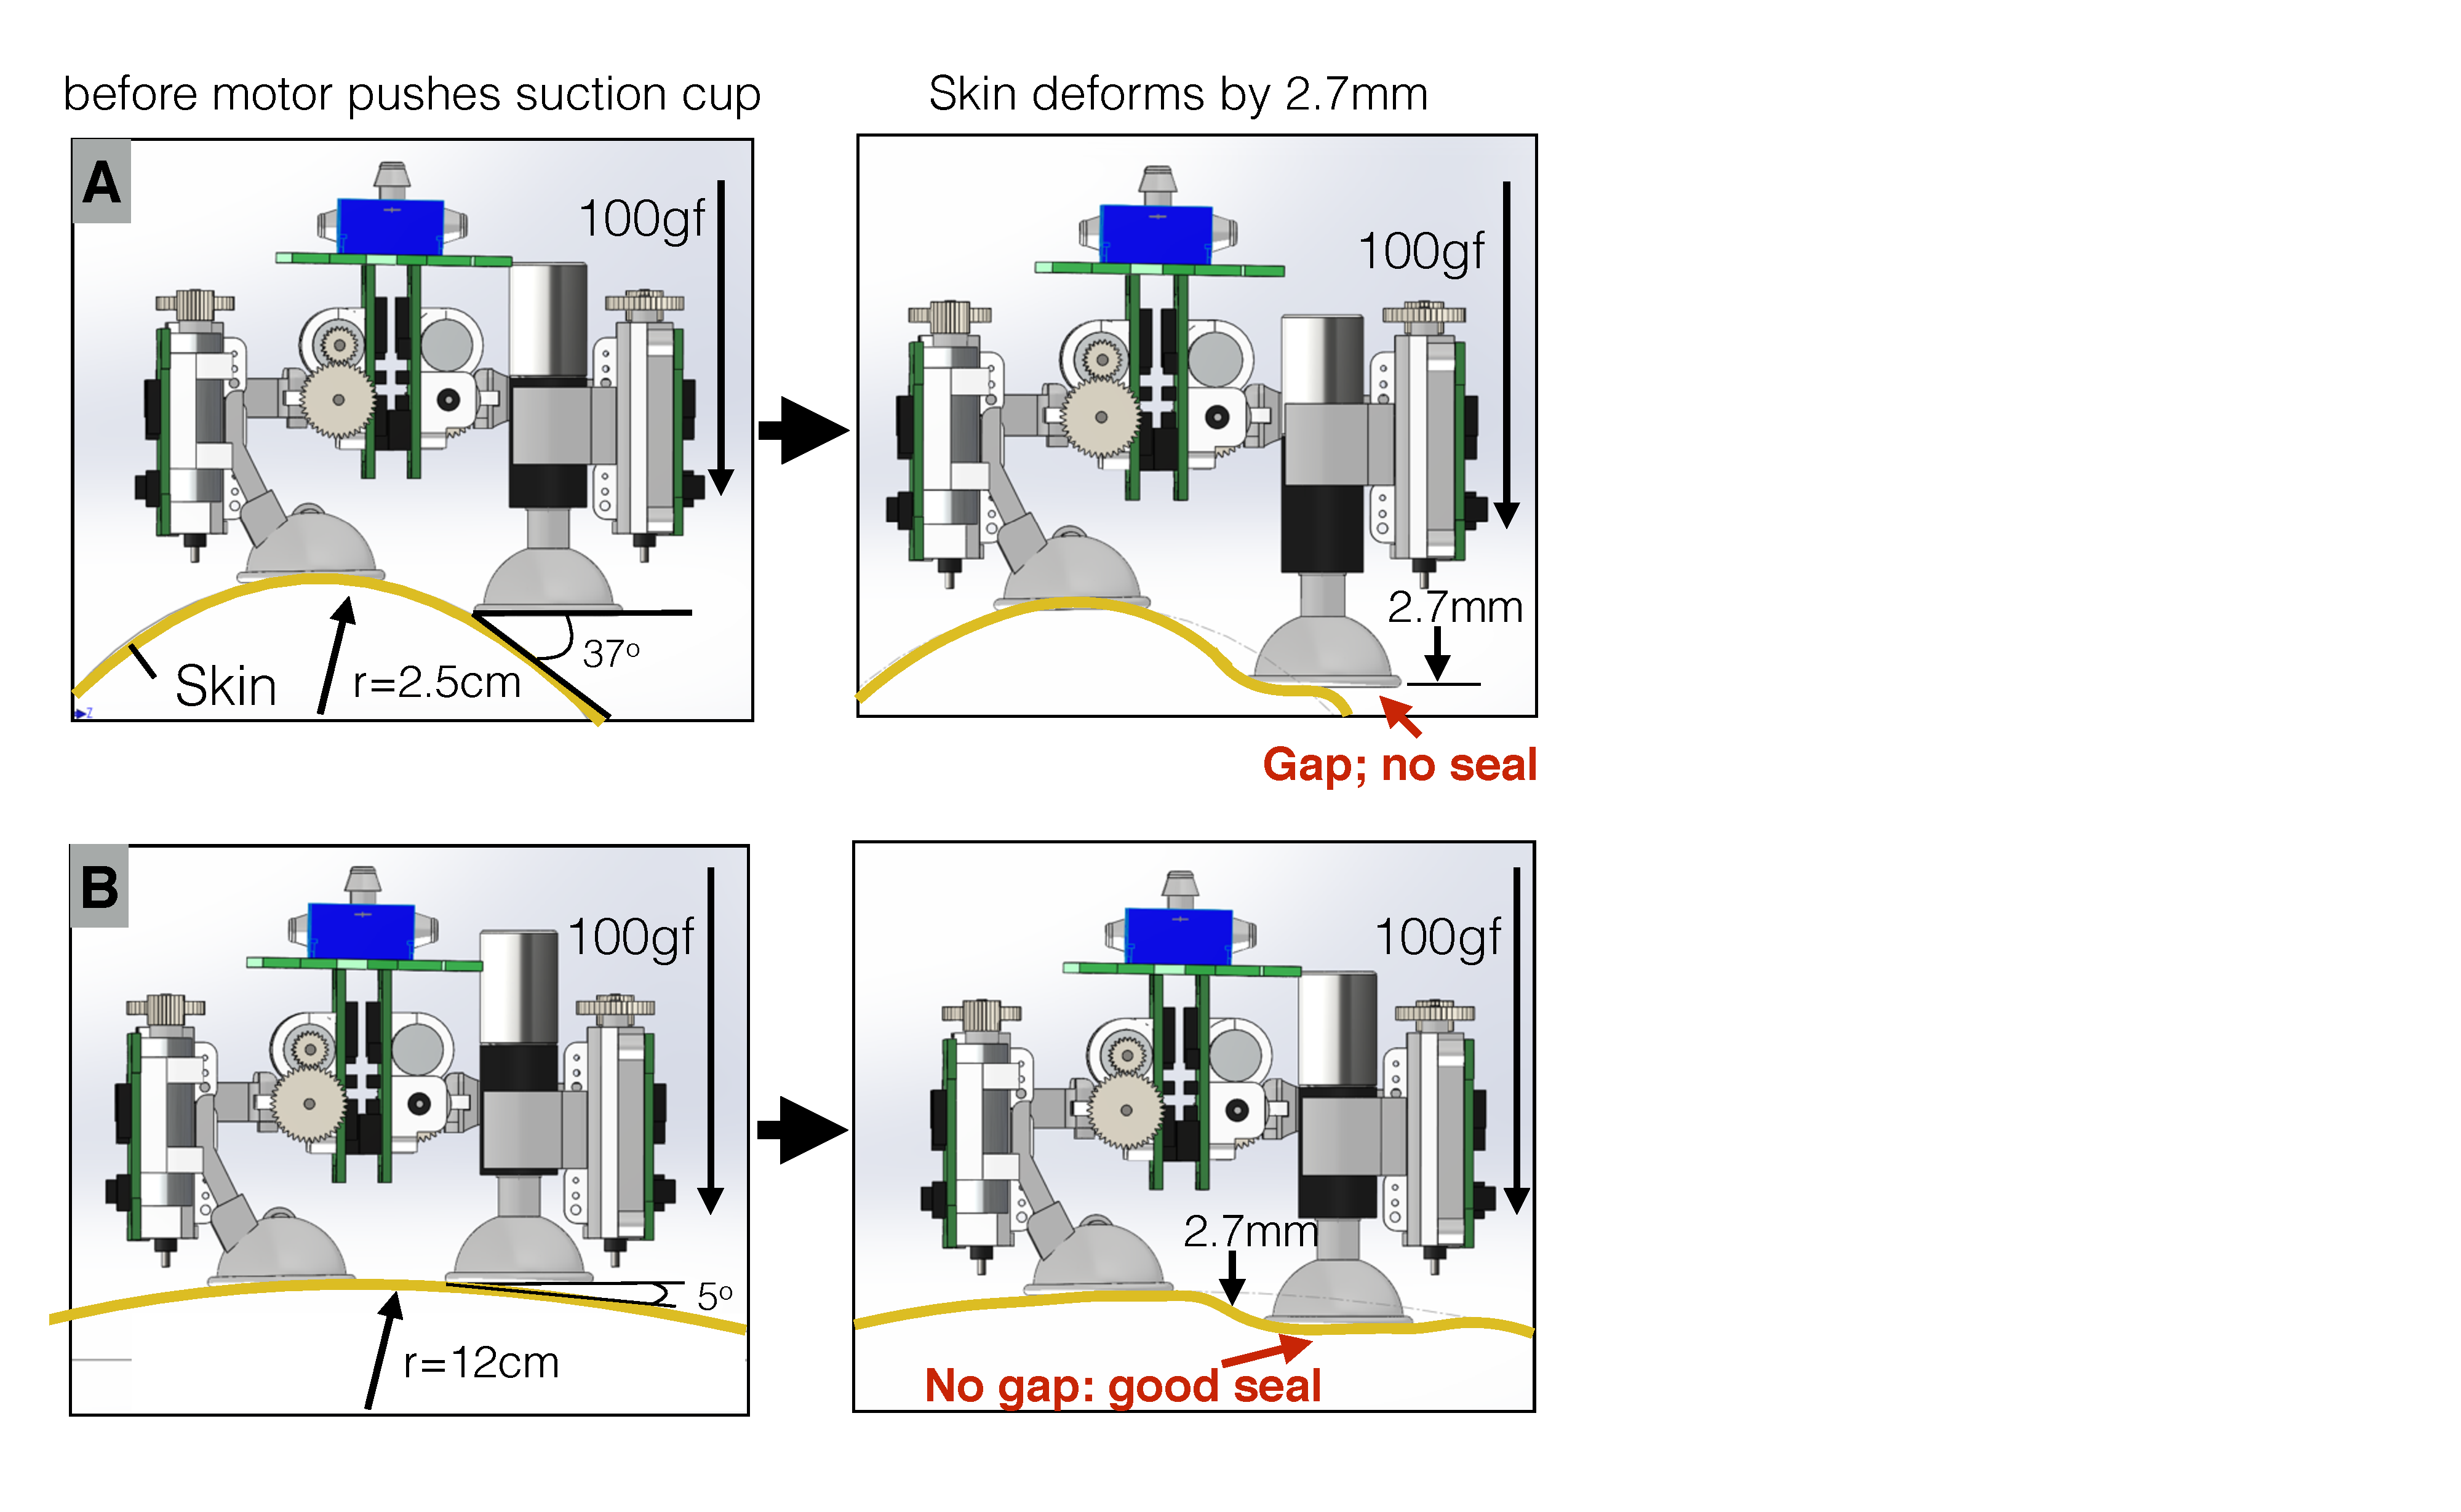
\includegraphics[width=8.9cm]{pictures/chapter3/curved_surface_attach.pdf}
\caption{Attachment to a curved skin. A)~Robot attachment to a cylindrical surface with a 2.5cm radius. Left: robot before it engages the vertical servo motor to push the suction cup down. Right: suction cup displaces the skin by about 2.7mm, which is not enough to make a reliable cup-skin seal. B)~Robot attachment to a cylindrical surface with a 12.5cm radius. In this case, a reliable cup-skin seal is created.}
\label{fig:surved_surface_attach}
\end{figure}

\subsection{Skin Curvature}
The human body has many degrees of curvatures, which may negatively affect the locomotion of SkinBot. To facilitate the analysis of curvature, previous studies have approximated the body with spheres and ellipsoidal cylinders~\cite{clauser1969weight}. In this work, we simplify each of the body parts with cylinders. In particular, we use cylinders with radii from 2.5cm (wrist-size) to 12cm (torso-size) to help cover some of the main adult-sized areas in which we envision SkinBot exploring. Ideally, suction cups should always be normal to the skin to maximize attachment. However, this may be challenging for cylinders with a small radius (i.e., a high degree of curvature) as the suction cups cannot reliably create the skin-cup seal. In our design, the suction cup is pushed towards the skin, causing indentation and allowing attachment with some degree of skin curvature. In particular, the skin can compress by 2.7 mm (SD: $\pm$0.71) when pushed by the linear servo motor before the motor stalls. Figure~\ref{fig:surved_surface_attach} shows a visualization of this process. The skin compression distance can be affected by many factors such as skin thickness and its elasticity. Theoretically, a 2.7mm compression distance allows an attachment to a minimum of 4.4 cm radius cylinders or a 1$5^o$ angle between the skin and the suction cup. To confirm this, we tested the robot on silicone (EcoFlex 00-30, thickness = 3.0 mm) placed over various 3D-printed cylinders and obtained similar results. In the future, the attachment to curved surfaces could be improved by adding the ability to pivot the suction cups to at least 37$^o$ so it can attach to 2.5 cm cylindrical surfaces. Alternatively, the robot locomotion mechanism could be shrunk by a factor of 2.2, from 9.1mm to 4.1mm distance between the centers of the suction cups to help circumvent smaller skin features. 

\begin{figure}[!t]
\centering
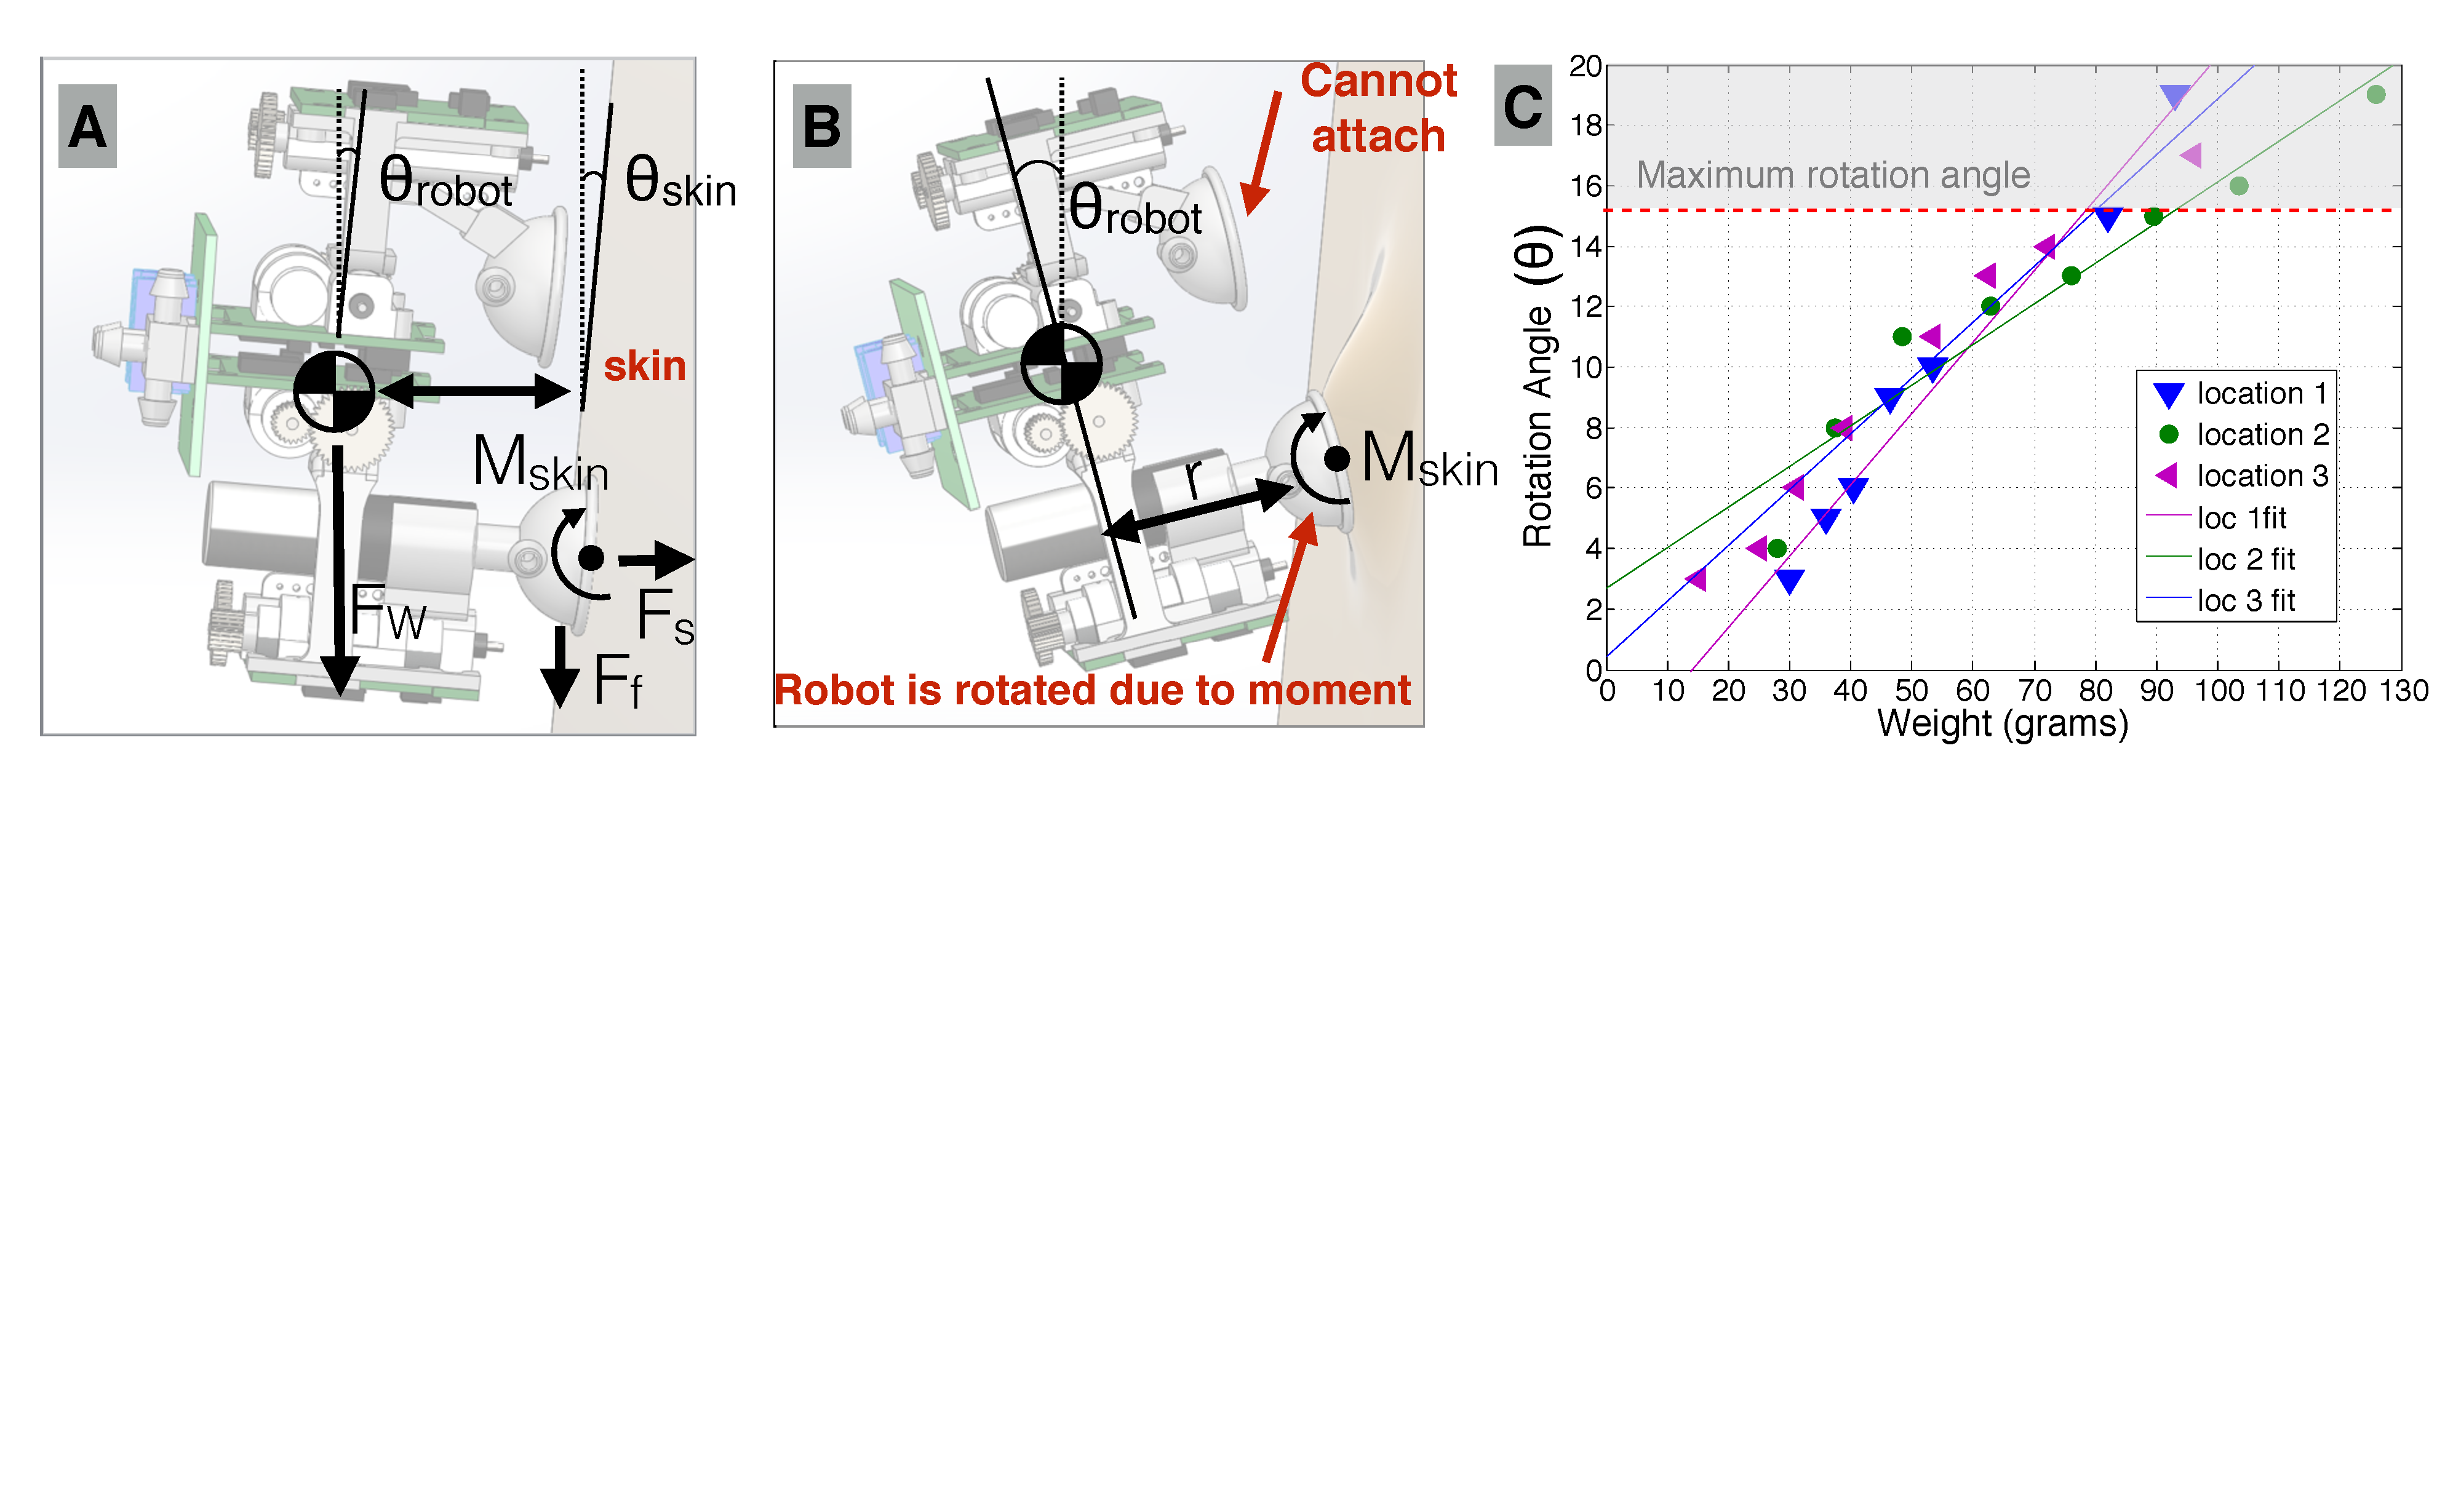
\includegraphics[width=14cm]{pictures/chapter3/sagging_exp.pdf}
\caption{Rotation of the robot due to sagging of the skin. A)~Free force diagram of the robot in a vertical position. One foot is detached, as the robot is taking a step. B)~An example scenario where the robot is rotated in a position that does not allow attachment. This is caused by sagging of the skin caused by torque ($M_{skin}$) on the skin, due to the weight of the robot. C)~The experimental data from three locations on the arm. The data shows the relationship between the robot rotation angle ($\theta_{robot} - \theta_{skin}$) and its weight. Linear fitting lines are shown.}
\label{fig:sagging_exp}
\end{figure}

\subsection{Skin Sagging}
Skin is stretchable and flexible surface, so it can affect the robot locomotion and orientation. These properties can create situations in which the skin sags, thus rotating the robot into unfavorable orientations. Figure~\ref{fig:sagging_exp}B, for instance, shows an example in which the robot is unable to attach the suction cup to the skin. Sagging is caused by the moment on the skin created by the weight of the robot. As determined in the previous section, the robot cannot reattach if the suction cup angle is larger than 15$^o$ in relation to the skin. To fully understand how the weight of the robot creates skin sagging, we measured how different suction cups rotate at different moments. In particular, we determined that to keep the angle under 15$^o$, the weight of the robot should be under 80g (see Fig.~\ref{fig:sagging_exp}C).

As shown in Figure~\ref{fig:sagging_exp}A, the moment on the skin ($M_{skin}$) caused by the robot is defined as: 
 \[M_{skin}=rF_w,~and~F_w=mg,~so~M_{skin}=rmg\]
where $r$ is the distance to the center of mass of the robot, $F_w$ is the force due to the weight of the robot, $m$ is the mass of the robot, and $g$ is gravity constant. The rotational stiffness is defined as: 
\[k = M_{skin}/\theta,~where~ \theta = (\theta_{robot} - \theta_{skin})\]
where $\theta$ is the rotational angle of the robot in relation to the skin. It follows that the rotational angle depends on the following:  
\[\theta = M_{skin}/k \]
\[\theta = rmg/k\]
As in the above equation, the experimental data shows that $\theta$ changes linearly ($r^2$ = 0.96) with the weight of the robot. The slope is dependent on the rotational constant $k$. In turn, $k$ depends on the skin's dimensions and structure, as well as its Young's modulus. Constant $k$ varies for the three tested locations from 0.13 to 0.24. 

We used a digital force gauge and DSLR camera (Mark IV, Canon) to record and later analyze the rotation angle. 

\subsection{Suction Marks}
We noticed that the suction left visible marks on the skin. We investigated this undesirable effect further in Figure~\ref{fig:arm_effect}, by recording the marks with a camera. We believe marks were caused by fluid displacement in the tissue due to pressure from the suction cup rim~\cite{lanir1990vivo}. The duration of how long marks remained visible depending on how long suction was applied to the skin. In one participant, the marks disappeared in under 10 sec for 5 sec of suction, and under 1 minute for 10 and 30 seconds of suction. Even after 10 minutes of continuous suction, the marks disappeared in about an hour. In practice, the pumps would not operate continuously but will be duty cycled to conserve energy. 

\begin{figure}[!t]
\centering
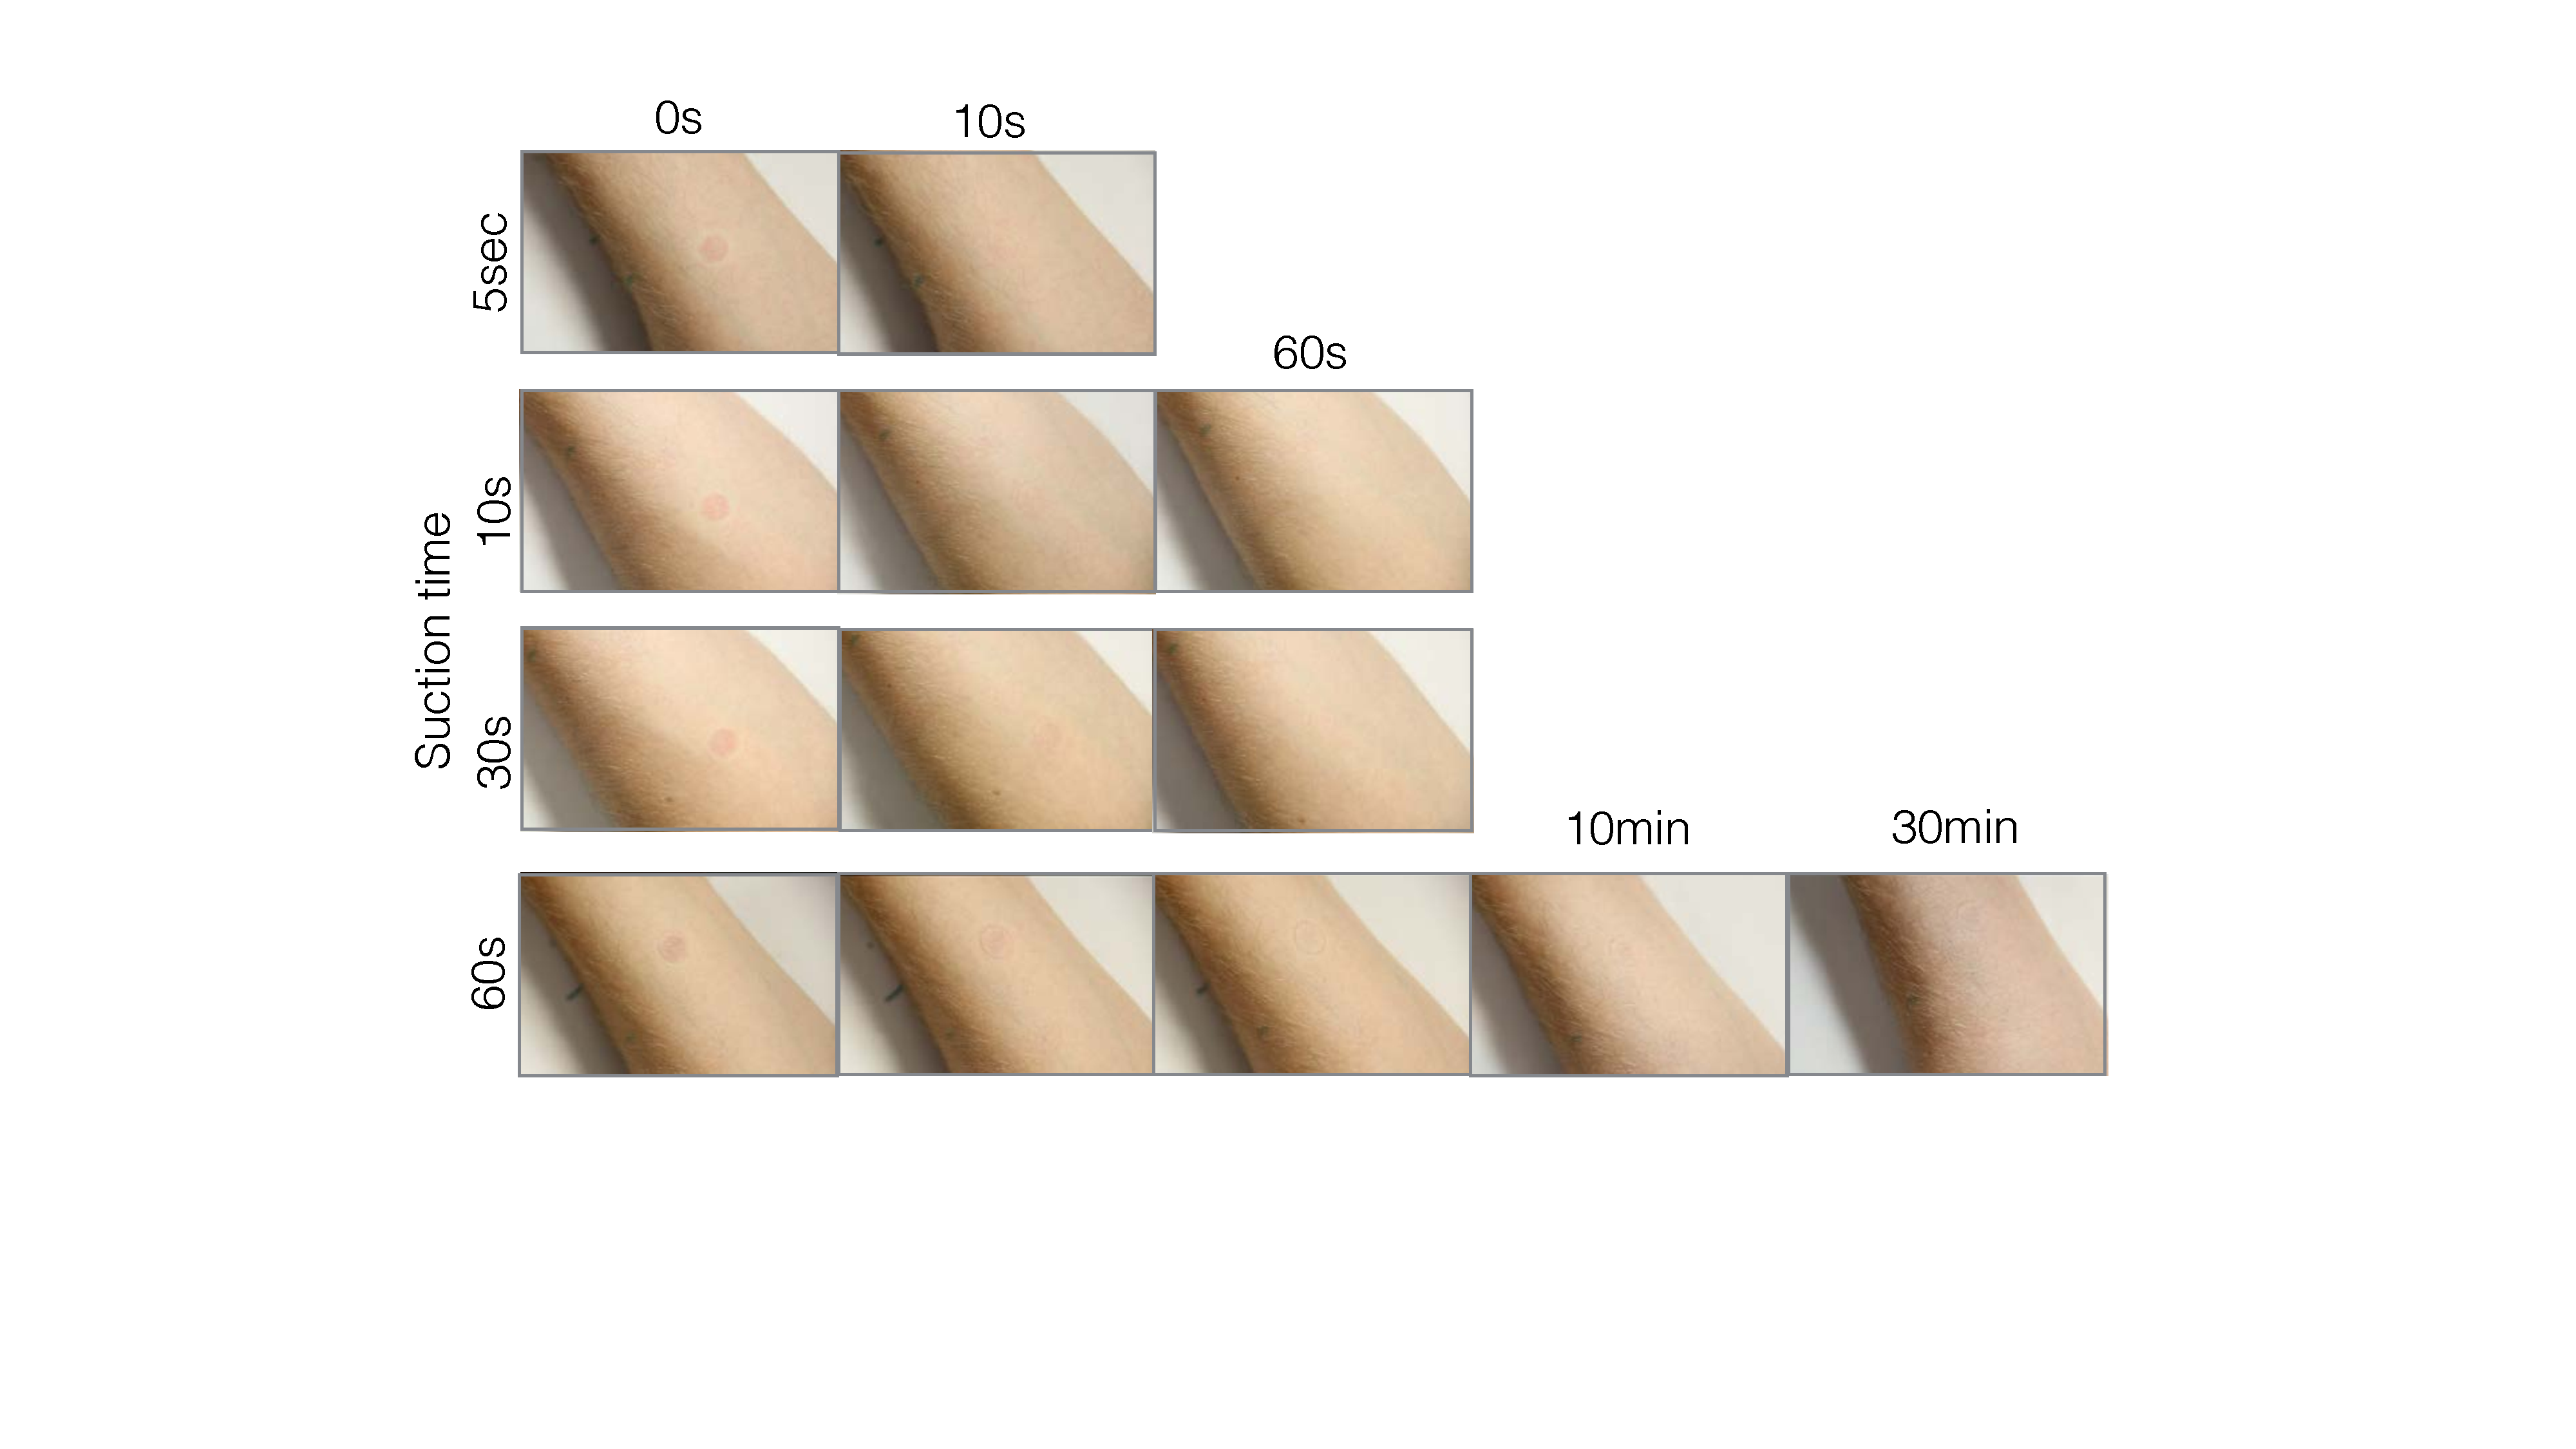
\includegraphics[width=12.0cm]{pictures/chapter3/arm_effect.pdf}
\caption{The after effect of the suction cups on the skin. The Y-axis is the duration the suction cup was applied to the skin. The snapshots are shown at different time intervals after the suction cup was removed. For example, when the suction cup was applied for 5 sec, no visible marks remained after 10 seconds.}
\label{fig:arm_effect}
\end{figure}

\section{Discussion}
Irrespective of the adhesion mechanism, epidermal robots need to have the following: a sensor to detect adhesion state, the ability to enable and disable adhesion, and at least two degrees of freedom (preferably, three) for the end effectors. To control skin locomotion, those three features need to be combined with a digital state machine. Commonly explored robot locomotion methods such as wheels and tracks do not perform well on the skin. Skin locomotion is difficult but possible with the use of sensors, feedback, and digital electronics. 

We determined that suction is an appropriate method for skin locomotion. Suction provides enough force to hold the robot, even with the moderate presence of hair. Highly dense hair would have to be shaved beforehand. Also, suction can be energy efficient, given that the pumps are duty cycled. Notably, for suction based robots, the weight should not exceed 80g to minimize skin sagging. The diameter of the suction cups should be under 10mm if -10 to -30kPa vacuum pressure is used. Also, the distance between suction cups should be ideally less than 4.1mm to facilitate locomotion over most curved body surfaces. Finally, adding a thin, soft rim to the rigid suction cup will aid in adhesion to skin with hair. 

%%-----------------ROVABLES ADHESION-----
\section{Cloth climbing}
This section shortly describes climbing on the clothing. Generally, the magnet mechanism in Rovables worked well, and it is miniature enough for an untethered robot. As a result cloth climbing does not require an in-depth study. 

It is crucial to quantify the force that Rovable can pull and how it is influenced by the type of fabric. This determines how much extra weight it can carry, which enables interactions such as actuating clothing. 

The force of attraction between wheels and the magnetic rod mostly depends on the thickness of clothing, as shown in Figure~\ref{fig:forces} (top). The measurements indicate the minimum force needed to pull wheels and magnet rod apart. Generally, thicker clothing has lower attraction forces. The maximum force is 4.2N when there is no clothing in between. Measurements were done with Series 5 force gauge (Mark-10). 

The minimum force required for climbing depends both on the thickness and type of fabric, as well as the weight of the robot. The thickness is dominant, but for some materials like linen, the climbing force does not follow the trend because of the low friction coefficient. Figure ~\ref{fig:forces} (bottom) reflects the force with the motor running at 3.7V DC on a horizontal plane. Its payload when going vertically will be the measured force minus its own weight, which is 0.2N. 

\begin{figure}[h]
\centering
  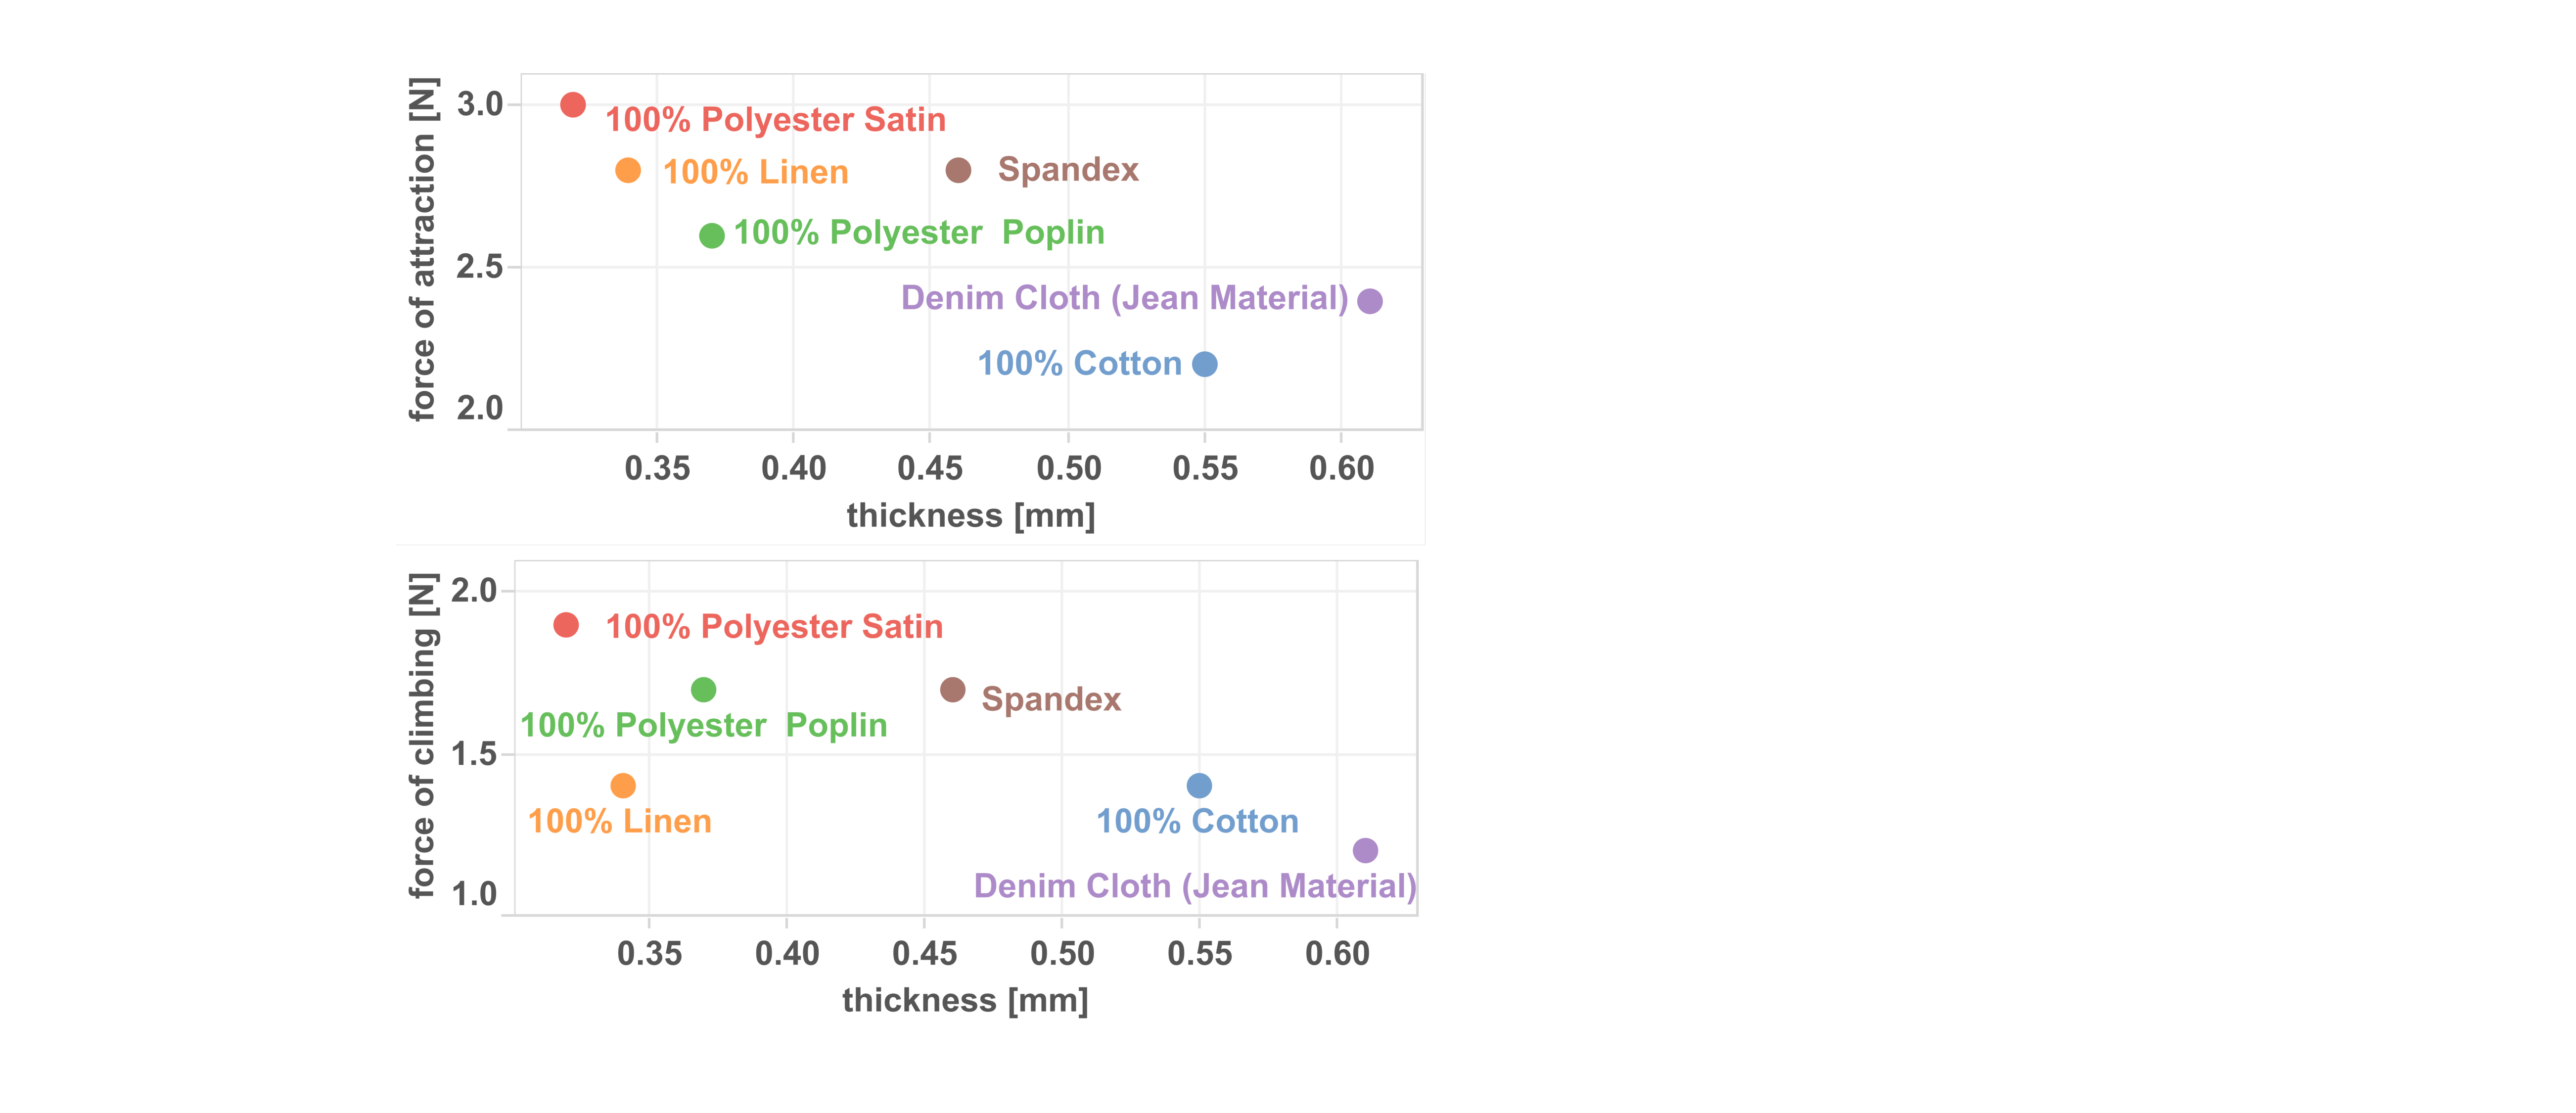
\includegraphics[width=0.8\columnwidth]{pictures/chapter4/forces_graph.pdf}
  \caption{Measurement of attraction~(top) and climbing forces~(bottom) on different fabrics. }~\label{fig:forces}
\end{figure}

\section{Summary}
%locomotion is hard 
% best is soft robotics 
Climbing is one of the biggest challenges for DWT robots. In this work, we have explored in detail how to attach and climb on the skin. The exploration showed that the skin is a complex and challenging surface. Cloth climbing is simpler than skin climbing. The cloth has uniform material properties and thickness and can be held by the backside with a magnetic force. 